\documentclass[../../main.tex]{subfiles}

\begin{document}

\chapter{CostCompiler}
CostCompiler é un interprete per il linguaggio di programmazione definito nel capitolo precedente Grammatica \ref{sec:grammatica}. Una volta ricevuto il programma, CostCompiler procede alla verifica e correttezza sintattica e semantica del programma, successivamente si occupa della generazione dell'albero di sintassi astratta. 
Questo albero rappresenta una versione astratta del programma, che astrae i dettagli sintattici del codice e si concentra sulla sua struttura logica, associando ad ogni costrutto (eg.\textit{if-then-else} un unico nodo, \textit{IfNode} presente nel omonimo file in src/ast).
Dopo aver generato l'albero di sintassi astratta,CostCompiler si della verifica Semantica \ref{sec:semantica} del linguaggio andando ad effettuare dei controlli semantici e di tipo sul programma in input, andando a garantire alcune invarianti.

Una volta effettuata la verifica semantica, CostCompiler procede con la generazione delle equazioni di costo, andando a visitare l'AST secondo determinati criteri, e che ad ogni nodo figlio verrá mandato una Map che contiene la mappatura di ogni variabile in una stringa che sará la stessa stringa che apparirá nelle equazioni di costo.\\
Ogni nodo figlio tornerá al padre attraverso la funzione \textit{toEquation()} che ritorna una stringa, rappresentante l'equazione di costo del nodo figlio, e il padre andrá a concatenare le stringhe dei figli(anche in base al tipo di figlio da cui ricevere l'equazione), ad esempio la \textit{return $<$EXP$>$ } sará diverso dal \textit{return }$<$function$(Par)>$.

Il risultato finale di questo processo di concatenazione attraverso determinati nodi dell'AST è la generazione delle equazioni di costo. 
Una volta generate le equazioni di costo, CostCompiler le stampa in un file \textit{equation.txt} inoltre lancerá il risolutore PUBS \ref{sec:pubs} che andrá a calcolare gli upper bound del programma da stampare a video.
Riportiamo un esempio di equazione di costo generata da CostCompiler dato un programma scritto in HLCostLang:
    \begin{lstlisting}[language=Java, caption={Listing8}]
    struct Params {
        address: array[int],
        payload: any,
        sender: string
    }
    service PremiumService : (string) -> void;
    service BasicService : (any) -> void;
    (isPremiumUser: bool, par: any) => {
        if ( isPremiumUser ) {
            call PremiumService("test");
        } else {
            call BasicService( par);
        }
    }
\end{lstlisting}
Una volta preso in input Listing8, CostCompiler genera le seguenti equazioni di costo:
\begin{lstlisting}[language=Java, caption={Equazioni di costo per Listing8}]
eq(main(P,ISPREMIUMUSER0,B),0,[if9(ISPREMIUMUSER0,P,B)],[]).
eq(if9(ISPREMIUMUSER0,P,B),nat(P),[],[ISPREMIUMUSER0=1]).
eq(if9(ISPREMIUMUSER0,P,B),nat(B),[],[ISPREMIUMUSER0=0]).
\end{lstlisting}
Andando a descriverle ci troveremo ad avere una equazione per la regola \textit{init}, dove vediamo che \textit{main} viene chiamata con costo 0 e verrá chiamata \textit{if9} con parametri \textit{ISPREMIUMUSER0,P,B}.
$P$ e $B$ sará il costo costante delle chiamate ai servizi \textit{isPremiumUser} e \textit{BasicService}, mentre \textit{ISPREMIUMUSER0} sará la valutazione del parametro \textit{isPremiumUser} che sará 1 se sará vero, 0 altrimenti; in altri termini \textit{ISPREMIUMUSER0} sará la valutazione della guardia del costrutto \textit{if-then-else} e verrá eseguita la chiamata al servizio \textit{PremiumService} se \textit{ISPREMIUMUSER0} sará 1 con costo $nat(B)$, altrimenti verrá eseguita la chiamata al servizio \textit{BasicService} con costo $nat(B)$. 
Una volta avere generato l'equazioni di costo dal programma, lo stampiamo in un file \textit{equation.txt}, cosi da poter eseguire PUBS(A Practical Upper Bounds Solver), per determinarci l'Upper Bound del programma.
L'obiettivo di PUBS(come vedremo in seguito \ref{sec:pubs}) è quello di ottenere automaticamente upper bound in forma chiusa per i sistemi di equazioni di costo, di conseguenza calcola i limiti superiori per la relazione di costo indicata come "Entry", oltre che per tutte le altre relazioni di costo di cui tale "Entry" dipende.
\section{Regole di Inferenza}
\label{sec:inference_rule}

I programmi di costo sono elenchi di equazioni che hanno termini:
$$f(\overline{x} ) = e + \sum_{i \in 0..n} f_i (\overline{e_i}) \quad \quad \quad \quad[\varphi ]$$
Dove le variabili si presentano nel lato destro e in $\varphi $ sono un sottoinsieme di $\overline{x}$; mentre $f$ e $f_i$ sono i simboli delle funzioni.
Ogni funzione ha un right-hand-side che è un'espressione aritmetica che può contenere:
\begin{itemize}
    \item Un'espressione in Presburger aritmetica (PA):
    $$e ::= x \quad | \quad q \quad | \quad e + e \quad | \quad e - e \quad | \quad q \cdot e \quad |  max(e_1,\dots,e_n)$$
    Dove $x$ è una variabile, $q$ è una costante intera, $e_1,\dots,e_n$ sono espressioni aritmetiche e $max$ è un operatore che restituisce il massimo valore tra le sue espressioni.
    \item Un numero di invocazioni di funzioni di costo: $f_i (\overline{e_i})$.
    \item La guardia $varphi$ é un vincolo congiuntivo lineare nella forma: $e_1 \geq e_2$ dove $e_1$ e $e_2$ sono espressioni aritmetiche di Presburger.
\end{itemize} 

La soluzione di un equazione di costo é il calcolo dei limiti di un particolare simbolo di una funziona(generalmente la prima equazione) e i limiti sono parametrici nei parametri formali dei simboli della funzione.
Definiamo un insieme di regole di inferenza che raccolgano frammenti di programmi di costo che vengono poi combinati in modo diretto dalla sintassi.
Usiamo una variabile di ambiente $ \varGamma $ come dizionari:
\begin{itemize}
    \item $\varGamma$ prende un servizio o un parametro e ritorna un espressione aritmetica di Presburger che di solito é una variabile.
    \item Quando scriviamo $\varGamma + i : \quad Nat $, assumiamo che i non appartenga al dominio di $\varGamma$.
\end{itemize}
I giudizi avranno forma:
\begin{itemize}
    \item $\varGamma \vdash e : Nat$ che significa che il valore di E in $e$ é rappresentato dalla costEspression $E$
    \item $\varGamma \vdash S : e ; C; Q $ significa che il costo di S nell'ambiente $\varGamma$ é $e + C$ dato un insieme di equazioni Q
\end{itemize}


\begin{align}
    &\mathrule{main}{
        \begin{aligned} \varGamma \vdash S : e ; C; Q  \quad \quad
        \overline{w} = \text{Var}(\overline{p},e) \cup \text{Var(C)}
        \end{aligned}
        }{\varGamma \vdash \overline{p}  \rightarrow \{S\}: 0 ;\emptyset;Q';C} \\
    &\mathrule{call}{\varGamma \vdash S : e ; C; Q}{\varGamma \vdash \text{call h}(\overline{E}) S : e + e' ; C; Q}\\
    &\mathrule{if}{
    \begin{aligned}
        &\varGamma \vdash E : \varphi  \quad \quad \varGamma \vdash S : e'; C; Q \quad \varGamma \vdash S : e"; C'; Q'\\
        &W = Var(e, e', e") \cup Var(C) \quad \quad \quad Q" =\big[ \begin{aligned}
            &\text{if}_l(\overline{w})  = e'+c[\varphi]\\
            &\text{if}_l(\overline{w})  = e"+c[\neg \varphi]\\
        \end{aligned}\big] \\
    \end{aligned}    
    }{\varGamma \vdash \text{if } E \text{ then } S_1 \text{ else } S_2 : 0; if_l(\overline{w}); Q; Q'; Q"}\\
    &\mathrule{let}{\varGamma + i : Not \quad \quad \quad \quad \overline{w} = Var(E) \cup Var(c)}{\varGamma \vdash \text{let } i = e \text{ in } S : S;e ; C; Q}\\
    &\mathrule{for}{
        \begin{aligned}
            &\varGamma \vdash M: e \quad \quad \quad \quad \varGamma \vdash i : Not\quad \quad \quad \quad \varGamma \vdash S : e'; C; Q\\
            &\overline{w} = Var(e, e') \cup Var(C) \ i \quad \quad \quad \quad Q' = \big[ \begin{aligned}
                &\text{for}_l(i,\overline{w}) = e + c\quad [i \lq e]\\
                &\text{for}_l(i,\overline{w}) = 0 \quad \quad [i \geq e]\\
            \end{aligned}\big]
        \end{aligned}
    }{\varGamma \vdash \text{for i in (0,M) } \text{ { S } } : 0; for_l(0,\overline{w}); Q; Q'}\\
\end{align}

Riassumiamo le regole descritte in precedenza:\\
\begin{itemize}
    \item Regola$[$call$]$ gestisce l'invocazione di un servizio; il costo della call sará il costo di $S$ piú il costo per l'accesso al servizio $h$ 
    \item Regola$[$if$]$ gestisce il costrutto condizionale;quando la guardi é un'espressione definita in aritmetica di Presburger e il costo verrá rappresentato da entrambi i rami con i due condizionali $\varphi $ e $\not \varphi$.\\Rappresentiamo a livello di equazione $if_l$ dove $l$ é la linea di codice dové inizia il costrutto.
    \item Regola $[$for$]$ descritto all'interno del rispettivo frammento di codice come $for_l$ per lo stesso motivo citato in precedenza; Definiamo i come Nat e verifichiamo che non sia presente nell'ambiente $\varGamma$ e scriviamo il rispettivo $S$ come caso base in cui $e \geq i$ oppure $i \geq e + 1$
    \item Regola $[$LetIn$]$ Dove viene definita E nell'ambiente $\varGamma$ con costo e(il costo per eseguire l'espressione $e$). Andremo a valutare se in $\varGamma$ é presente $E$ e andiamo a valutare $\varGamma \vdash S$ che ritornerá un'equazione $Q'$ con costo $C$.
\end{itemize}
\section{Generazione delle Equazioni di costo}
La generazione delle equazioni di costo viene eseguita andando a implementare le regole di inferenza viste in precedenza.
Ogni nodo all'interno del nostro AST conterrá il metodo \textit{toEquation()} che prende come argomento la variabile che nostro ambiente $\varGamma$ e sará appunto un dizionario.
Questo dizionario di tipo $EnvVar$ é un HashMap che contiene come chiave l'oggetto Nodo della variabile e come valore la stringa rappresentante.
Abbiamo deciso di utilizzare questo approccio per focalizzarci sull'efficienza del farci restituire la variabile che mappa quel determinato Nodo, senza dover andare a cercare all'interno dell'HashMap la chiave che mappa quel valore, cosa che viene fatta all'inserimento di un Nodo.
L'inserimento del nodo peró non sempre é un operazione onerosa per il fatto che abbiamo gia il controllo semantico che ci garantisce che non ci saranno variabili non dichiarate oppure variabili non dichiarate prima del loro utilizzo.

Andiamo ad analizzare un esempio semplice, all'interno del Nodo di tipo \textit{CallService.java} che rappresenta l'invocazione di un servizio, abbiamo il metodo \textit{toEquation()} che prende come argomento l'ambiente $\varGamma$ e restituisce una stringa che rappresenta l'equazione di costo del nodo, che sará un stringa riportata all'interno dell'equazione di costo del padre.

\begin{lstlisting}[language=Java]
    @Override
    public String toEquation(EnvVar e) {
        return "nat("+e.get(this)+")" + (stm!= null ? "+"+stm.toEquation(e) : "");

    }
\end{lstlisting}

La sezione $e.get(this)$ ritorna la variabile mappata per quel determinato nodo, che sará una stringa che rappresenta la variabile all'interno dell'equazione di costo, mentre la sezione $stm.toEquation(e)$ é la chiamata sul metodo \textit{toEquation()} del nodo figlio, che restituirá la stringa che rappresenta l'equazione di costo del nodo figlio.

Per avere una panoramica completa del processo di generazione delle equazioni di costo, riportiamo il frammento di codice di $toEquation()$ del $programNode$:
\begin{lstlisting}[language=Java]
    public String toEquation(EnvVar e){

        for (Node n : decServices){
            n.checkVarEQ(e);
        }
        StringBuilder equ = new StringBuilder();
        for(Node n : funDec){
            equ.append(n.toEquation(e));
        }
        equ.append(main.toEquation(e));
        return equ.toString();
    }
\end{lstlisting}

Come possiamo vedere, prima di generare le equazioni di costo del programma, andiamo a controllare che le variabili dichiarate all'interno dei servizi siano presenti all'interno dell'ambiente $\varGamma$ e le mappiamo con determinate stringhe che appariranno nelle equazioni, successivamente andiamo a iterativamente all'interno delle singole funzioni le generiamo e le concateniamo alla stringa che rappresenta le equazioni di costo del programma.
Infine ci occupiamo di generare le equazioni di costo della funzione main, che saranno concatenate anch'esse con la stringa che rappresenta le equazioni di costo del programma.


\section{PUBS}
\label{sec:pubs}
Pubs é un risolutore di vincoli di costo, che prende in input un file di equazioni di costo e restituisce un file con i limiti superiori per ogni relazione di costo.
PUBS (Pratical Upper Bounds Solver) ha l'obiettivo di ottenere automaticamente upper bound in forma chiusa per i sistemi di equazioni di costo, di conseguenza calcola i limiti superiori per la relazione di costo indicata come "Entry", oltre che per tutte le altre relazioni di costo di cui tale "Entry" dipende.
Nell'output di pubs vengono mostrati anche i passaggi intermedi eseguiti che coinvolgono il calcolo delle funzioni di classificazione e degli invarianti di ciclo.

\begin{figure}[H]
    \centering
    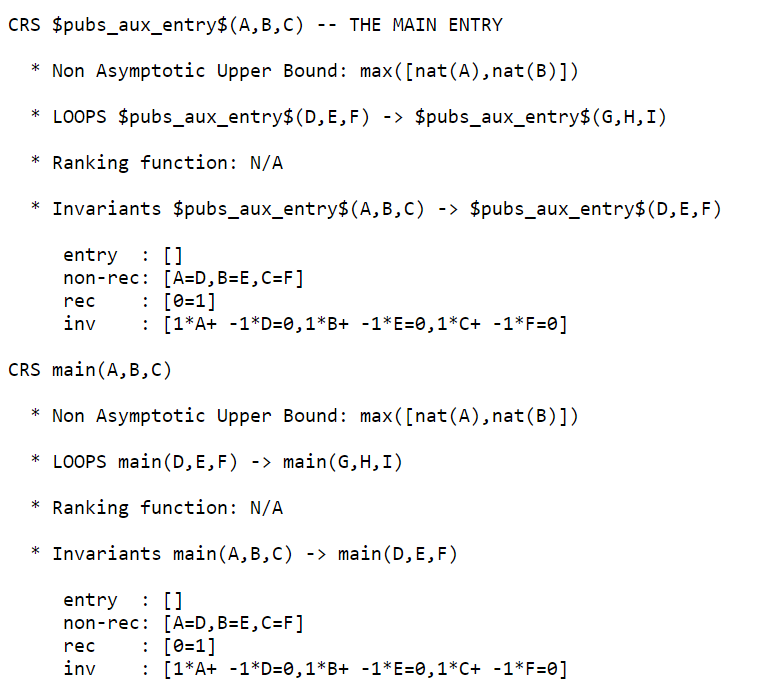
\includegraphics[width=0.9\textwidth]{pubs_example.png}
    \caption{Esempio di output PUBS su Listing 1}
\end{figure}
Come vediamo nell'immagine sopra, PUBS ci restituisce un analisi dell'intera equazione ($pub\_aux\_entry$) e delle singole funzioni da cui essa dipende, in questo caso $pubs\_aux\_if9$ e $pubs\_aux\_main$.
In questo caso con ``Listing1'' abbiamo un Upper Bound non Asintotico di $max(Nat(A), Nat(B))$ che ci determina che il costo del programma dipende dalle variabili A e B, e che il costo del programma sará il massimo tra i due.
Inoltre non abbiamo la presenza di cicli, quindi PUBS non ci restituisce nessun invariante di ciclo.

In PUBS peró abbiamo una grammatica da rispettare, tenuta in considerazione da ogni equazione di costo generata da CostCompiler, che é la seguente:
\begin{lstlisting}[language=Java, caption={Grammatica PUBS}]
    <equation> ::= eq(Head,costExpression,[listOfCall],[ListOfSizeRelation]).
    <Head> ::= Name | Name(Par).
    <costExpression> ::= nat(<variable>) 
                    | <costExpression> + <costExpression> 
                    | <costExpression> - <costExpression> 
                    | <costExpression> * <costExpression> 
                    | max(<costExpression>,<costExpression>).
                    
    <listOfCall> ::= [] | <call> <listOfCall>.
    <call> ::= <function>(<listOfParameters>).
    <listOfParameters> ::= [] | <variable> <listOfParameters>.
\end{lstlisting}
Dove $<$Head$>$ é il nome della entry che andremo ad analizzare insieme a i suoi parametri.
CostExpression é l'espressione di costo che rappresenta il costo della entry, come notiamo rispetta la grammatica della aritmetica di Presburger.
ListOfCall é la lista delle chiamate alle altre entry, che saranno rappresentate come $<$call$>$ e $<$listOfCall$>$ sará la lista di queste chiamate; in questo modo PUBS riesce a costruire un grafo delle dipendenze tra le entry.
Infine abbiamo $<$listOfSizeRelation$>$ che sará la lista delle relazioni di costo che dipendono dalla entry che stiamo analizzando, e che PUBS andrá a calcolare.
Riportiamo Listing1 come esempio di equazione di costo generata da CostCompiler, dove troviamo l'analisi alla pagine precedente:
\begin{lstlisting}[caption={Equazione di costo PUBS per Listing6}]
    eq(main(B),1,[svc(B)],[]).
    eq(svc(B),0,[for3(0, B)],[] ).
    eq(for3(M, B) ,nat(B),[for3(M+1, B)], [10>= M]).
    eq(for3(M, B) ,0,[],[M >= 10+ 1]).
\end{lstlisting}

Nella prima riga troviamo l'entry $main$ che prende in input B, con costo 1, chiama la funzione $svc$.
Quest'ultima andrá a chiamare la funzione $for3$ inserendo un'ulteriore parametro che sará il counter del ciclo con parametro 0 e B, che avrá costo 0 in caso $M >= 10 + 1$ altrimenti avrá costo $nat(B)$. 
\end{document}